\section{The Dopler Effect and Special Relativity}

Consider the case of a stationary observer and a source that is moving away with some velocity $v$ i.e. the velocity of recession, $\Delta S$ is the period of wave at source, $\Delta t_O$ is the period of the wave at observer. The source emits a wave in some medium which travels at speed $u$. We want the relationship between the $t$'s.

\begin{figure}[h!]
    \centering
    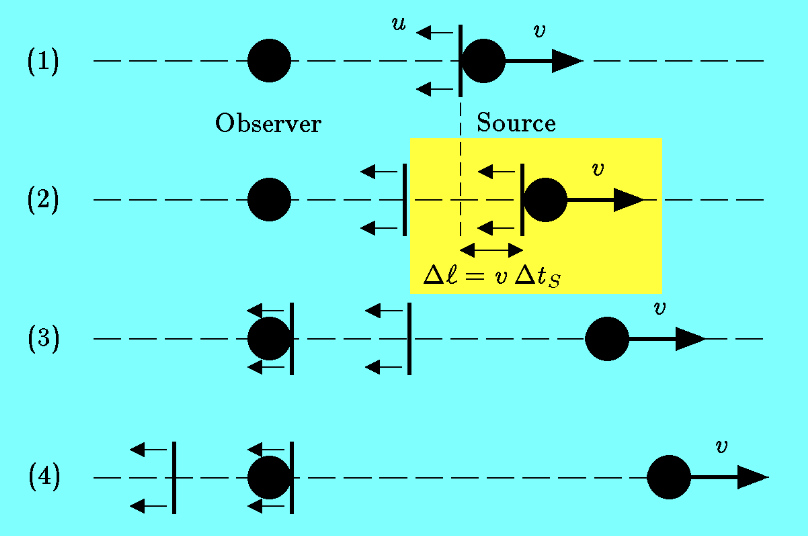
\includegraphics[width=0.5\textwidth]{images/doppler 1.png}
    \caption{Non-relativistic case. Source moves away from observer.}
\end{figure}

\begin{enumerate}[label=(\arabic*)]
    \item The source is emmiting a wave crest
    \item the source emits a second wave crest, but it also has moved. The highlighted part shows that the second wave crest has to move a bit more than the first one. This is what accounts for the Doppler effect. Here $\Delta l$ is the crucial quantity
    \item The waves have traveled and the first crest has hit the observer
    \item The second crest has hit the observer.
\end{enumerate}

To figure out the Doppler shift, realise that if both objects were stationary then their periods would coincide i.e. $t_O = t_S$. But since there is motion, the second crest will have to travel further by $\Delta l$, so

\begin{equation*}
    \Delta t_O = \Delta t_S + \frac{\Delta l}{u} = \Delta t_S + \frac{v \Delta t_S}{u} \quad \Rightarrow \quad \frac{\Delta t_0}{\Delta t_S} = 1 + \frac{v}{u} = \frac{\lambda_O}{\lambda_S} = 1 + z
\end{equation*}
where $\lambda_S$ and $\lambda_O$ are the wave wavelengths for source and the oberver correspondingly, $z$ is \textbf{the redshift.} Note that $z=0$ corresponds to stationary situation i.e. no redshift. In this case 

\begin{equation*}
    z=\frac{v}{u} \qquad \text{Nonrelativistic, source moving} 
\end{equation*}

Now let's consider a different case, where the observer is moving with velocity $v$ and the source is stationary.

\begin{figure*}[h!]
    \centering
    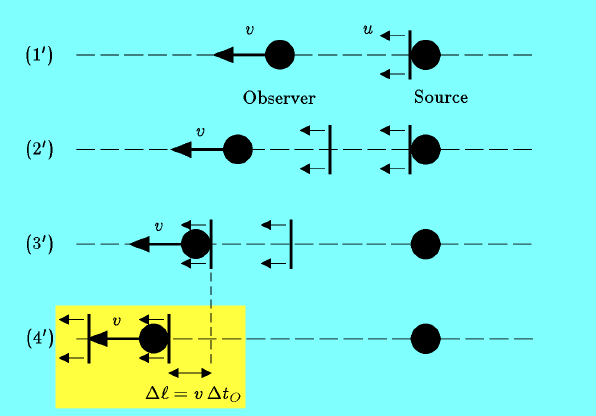
\includegraphics[width=0.5\textwidth]{images/doppler 2.png}
    \caption{Non-relativistic case. Observer moves away from the source}
\end{figure*}

\begin{enumerate}[label=(\arabic*')]
    \item Again, first wave crest is emited
    \item The second wave crest is emited by the source
    \item The first wave crest arrives at the source
    \item The second wave crest arrives at the source. In this case this is the most important frame. At the moment the second wave crest reaches the observer, the observer has moved by a distance $\Delta l$
\end{enumerate}

So similarly, is there was no motion then $\Delta t_O = \Delta t_S + \frac{\Delta l}{u} = \Delta t_S + \frac{v \Delta t_O}{u}$. Solving this equation we obtain

\begin{equation*}
    \frac{\Delta t_O}{t_S} = \left( 1 - \frac{v}{u} \right)^{-1}
\end{equation*}
Hence the redshift

\begin{equation*}
    z = \frac{\Delta t_O}{\Delta t_S} - 1 = \left( 1 - \frac{v}{u} \right)^{-1} -1 = \frac{v/u}{1 - v/u} \qquad \text{Nonrelativistic, observer moving}
\end{equation*}

Note that

\begin{equation*}
    z_{\text{O moving}} - z_{\text{S moving}} = \frac{(v/u)^2}{1-(v/u)}
\end{equation*}
Note that this shows more explicitly that z is proportional to the square of $v/u$. If we had a small $v/u$ then the denominator would vanish. Also note that this does not break the galilean relativity, but when we transform into another frame we get that the air is moving i.e. when we say that something is at rest, it is at rest to the medium that is transporting the wave. Let's move to the relativistic case.

We will consider three effects of special relativity:
\textbf{Time dilation.} Any clock which is moving at speed $v$ relative to a given frame will "appear" (to an observer using that reference frame) to run slower than normal by a factor $\gamma$, and given by

\begin{equation*}
    \gamma \equiv \frac{1}{\sqrt{1 - \beta}}, \qquad \beta \equiv v/c
\end{equation*}
Notice that for $v \ll c$ the effect is small and $\gamma \simeq 1$, meaning that effectively there is no effect. The word "appear" is a subtle term. When we say it, we don't mean that we litteraly see the clock running slower, since seeing just means that we're measuring the light pulses as they arrive with our eyes and since light has finite travel time, that means that we measure things at different times. Suppose a large object is coming towards you, you would be seeing the back at an ealier time (the light travels longer) than the front. So the problem is that we're seeing different pieces of it at different times, in terms of the actual existance of the thing. So in order to know what we're \textbf{seeing} we would need to calculate point by point what you would be seeing for every part of the object. The simple expressions like the one above are based on what a \textbf{frame of reference sees}. And a frame of frame of reference we consider as a structure of ruler and with clocks located everywhere in that grid (all of which have been synchronized to start with). And if you want to know at what time an event happens you look at the clock next to it. And when we compare how the local clocks would compare, we see this time dialation effect (taking out the light travel time). In regards to the relativistic doppler shift, we'll see that the clock coming towards the observer is running \textbf{faster} and this happens becouse the distance gets smaller beating the effect of time dilation. To recover regular time dilation we would need moving clocks speed be perpendicular to the observer, meaning that the photon going from the clock would need to be perpendicular to the travel velocity of the clock wrt the observer.

Now, doing the calculation we assume that the wave is a light wave and the velocities are comporable to $c$ i.e. time dilation effect is important enough and we want to take it into account. Now we would expect to get the same results, regardless if the observer or the source is moving. Since previously, it was the air that was not stationary anymore when we transformed into another reference frame.

It is crucial that what we talk about things measures from a particular reference frame, since the transformation from one reference frame to another is non-trivial. So the time between the pulses as measured from the source clock is what we call $\Delta t_S$. The source (effectively a clock since it's emmiting pulses at regular intervals which fits in the definition of a clock) is moving in this picture, so relative to our frame (again we always think of properties as being consistent in our frame), it's clock will be running slower by a factor of gamma. And since the observer is not moving there is no time dilation associated with the observer.

\begin{figure*}[h!]
    \centering
    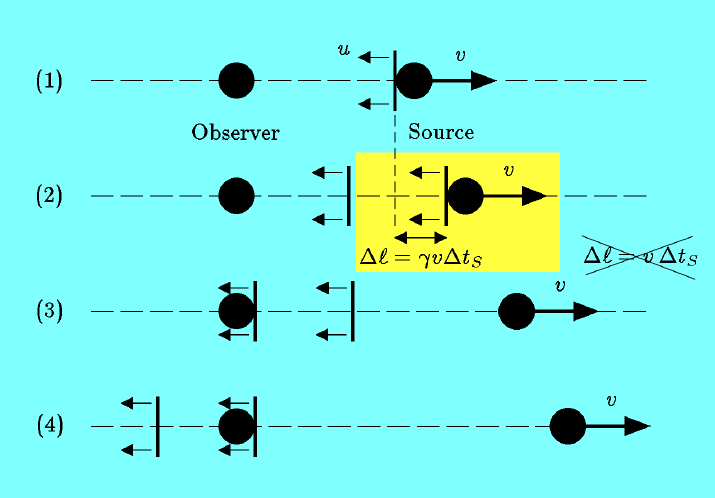
\includegraphics[width=0.5\textwidth]{images/doppler 3.png}
    \caption{Relativistic case. Source moves away from the observer}
\end{figure*}

\begin{equation*}
    \Delta t_O = \gamma \Delta t_S + \frac{\Delta l}{u} = \gamma \Delta t_S + \frac{v \gamma \Delta t_S}{u} = \gamma \left( 1 + \frac{v}{c} \right) \Delta t_S
\end{equation*}
but note the difference of the squared in $\gamma$ factor.

\begin{equation*}
    \Delta t_O = \sqrt{\frac{1 + \beta}{1 - \beta}} \Delta t_S \qquad \text{Relativistic, source moving}
\end{equation*}

Next, we'll do the relativistic case of observer moving. Our frame of reference is the frame of reference of the image, so we'll see the observers clock running slower.

\begin{figure}[h!]
    \centering
    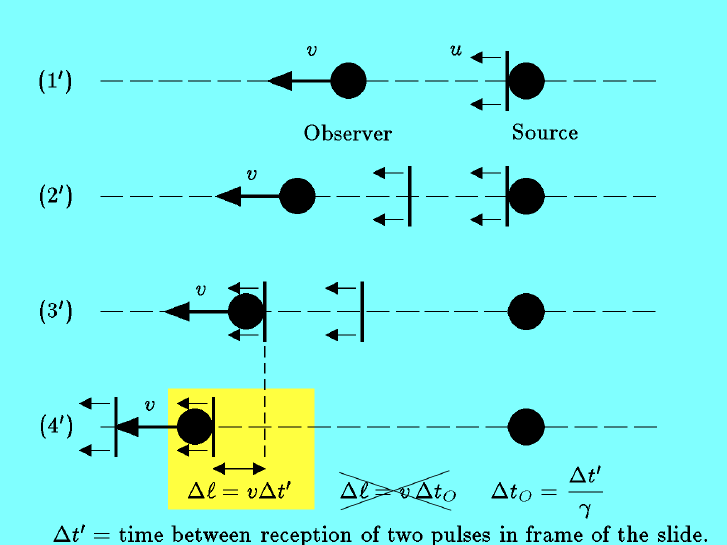
\includegraphics[width=0.5\textwidth]{images/doppler 4.png}
    \caption{Relativistic case, observer is moving}
\end{figure}

Again, we want everything in terms that we're measuring it. So the distance the observer moevd is its velocity times the time elapsed from frame (3') to frame (4'). This time our reference frame coincides with the reference frame of the source.

\begin{align*}
    & \Delta t' = \gamma t_O \quad \Rightarrow \quad \Delta t' = \Delta t_S + \frac{v \Delta t'}{c} \quad \Rightarrow \quad \Delta t' = \left( 1 - \frac{v}{c} \right)' \Delta t_S \\
    \Rightarrow \; &\Delta t_O = \frac{1}{\gamma} \left( 1- \frac{v}{c} \right)^{-1} \Delta t_S = \sqrt{(1+\beta)(1-\beta)} \frac{1}{1 - \beta} \Delta t_S
\end{align*}

\begin{equation*}
    \Delta t_O = \sqrt{\frac{1+\beta}{1- \beta}} \Delta t_S \quad \text{Relativistic, source or observer moving}
\end{equation*}

\begin{equation*}
    z = \frac{\Delta t_O}{\Delta t_S} - 1 \sqrt{\frac{1+\beta}{1-\beta}} - 1 \quad \text{Relativistic}
\end{equation*}

Special relativity only describes things happening only in inertial reference frames (uniform velocity). What about clocks that are accelerating? As long as gravity is absent we can use the dynamical equations of special relativity. The clock is a complicated system so to simplify matters we assume that the acceleration does not affect its speed. The assumption that we're making is that these are ideal clocks (built well and does not break under large accelerations) and for the "acceleration does not affect its speed" part we assume that the clock runs the exactly same as the clock running along side it at the same speed but with no acceleration. At every particular point during the motion of the clock the tick speed is effected by the motion by a factor of gamma, but we're assuming that it is the same as the effect of non-accelerating clock, meaning that there is no effect of acceleration.

Kinematic effects (3 and no more), are time dilation, which we have already seen. Second, is the Lorentz (-Fitzgerals) contraction: any rod which is moving at a speed $v$ along its length relative to a given reference frame will "appear" (to an observer using that reference frame) to be a shorter than its normal length by the same factor $\gamma$. A rod which is moving perpendicular to its length does not undergo a change in apparent length.

\begin{figure}[h!]
    \centering
    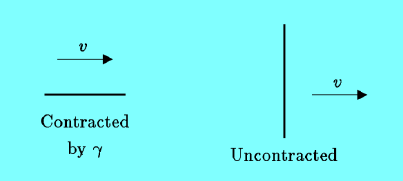
\includegraphics[width=0.35\textwidth]{images/lorentz contraction.png}
    \caption{Lorentz contraction}
\end{figure}

Next is the relativity of simultaneity: suppose a rod which has rest length $l_0$ is equipped with a clock at each end. The clocks acan be synchronized in the rest frame of the system by using light pulses. (That is, a light pulse can be sent out from the center, and the clocks at both ends can be started when they receive the pulses.) If the system moves at speed $v$ along it's length, the the traullling clock will "appear" to read a time which is later than the leading clock by and ammount $\beta l_0/c$. If, on the other hand, the system moves perpendicular to its length, then the synchronization of the clocks is not disturbed.

This is a crucial concept. Since on the first look it might seems like two observers moving relative to each other measure other's clock as ticking slower, however the concept of simultaneity would show that the clocks one reference frame would not be considered synchronised.